\documentclass[10pt,a4paper]{article}
\usepackage[latin1]{inputenc}
\usepackage{amsmath}
\usepackage{amsfonts}
\usepackage{amssymb}
\usepackage{graphicx}
\author{Antonio Jes�s Heredia Castilllo}
\title{Comparaci�n de resultados ejercicio 7}
\begin{document}
	\maketitle
	En este ejercicio vamos a comparar como funcionaria un kernel para sumar matrices en Cuda con diferentes modificaciones. 
	
	El c�digo original usara bloques 2D para sumar las matrices. En la primera modificaci�n usaremos bloques 1D donde una hebra sumara todas posiciones de una misma fila. Y en la segunda modificaci�n una hebra sumara todas las posiciones de la misma columna. El c�digo de estas modificaciones esta adjuntado junto al PDF. 
	Para ver como responde estas modificaciones haremos pruebas con distintos par�metros. \\
	El primer experimento lo hemos realizado con un tama�o de bloque de $8x8$ y matrices de distintos tama�os. Los datos obtenidos los podemos ver en la siguiente tabla: \\
	\begin{tabular}{|c|c|c|c|}
		\hline 
		N & Original & Modificaci�n 1 & Modificaci�in 2 \\ 
		\hline 
		40 & 0,000037 & 0,000045 &  0,000056 \\ 
		\hline 
		100 & 0,000089 & 0,000133 & 0,000096 \\ 
		\hline 
		200 & 0,000206 & 0,000211 &  0,000295\\ 
		\hline 
		500 & 0,001403 & 0,001081 & 0,001570 \\ 
		\hline 
		1000 & 0,004000 & 0,004133 & 0,006002 \\ 
		\hline 
		2000 & 0,015110 & 0,020209 & 0,022229 \\ 
		\hline 
		5000 & 0,096241 & 0,161487 & 0,177768 \\ 
		\hline 
		10000 & 0,360276 & 0,745313 & 0,665087 \\ 
		\hline 
		20000 & 0,699896 & 0,787172 & 0,753009 \\ 
		\hline 
	\end{tabular} \\\\
Y a continuaci�n podemos ver una grafica comparando los resultados. 
\begin{figure}[h]
	\centering
	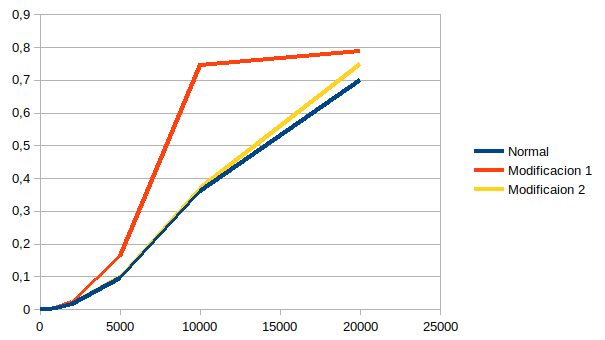
\includegraphics[width=0.7\linewidth]{screenshot002}
		\caption[Comparaci�n 8x8]{Comparaci�n 8x8}
	\label{fig:screenshot002}
\end{figure}

El siguiente experimento lo he realizado para tama�os de bloque de 16x16. Los resultados se pueden ver en la siguiente tabla: \\
\begin{tabular}{|c|c|c|c|}
	\hline 
	N & Original & Modificaci�n 1 & Modificaci�in 2 \\ 
	\hline 
	40 & 0,000034 & 0,000076 &  0,000149 \\ 
	\hline 
	100 & 0,000067 & 0,000138 & 0,000089 \\ 
	\hline 
	200 &0,000223& 0,000283 &  0,000230\\ 
	\hline 
	500 &0,001229 & 0,001267 & 0,001325 \\ 
	\hline 
	1000 & 0,004194 & 0,003891 & 0,004356 \\ 
	\hline 
	2000 & 0,018465 &0,024261 & 0,016769 \\ 
	\hline 
	5000 & 0,101747 & 0,170346 & 0,096955 \\ 
	\hline 
	10000 & 0,420579 & 0,654600 & 0,448342 \\ 
	\hline 
	20000 & 0,742035 & 1,012560 & 0,738639 \\ 
	\hline 
\end{tabular} \\\\
Y a continuaci�n podemos ver una grafica comparando los resultados. \\
\begin{figure}[h]
	\centering
	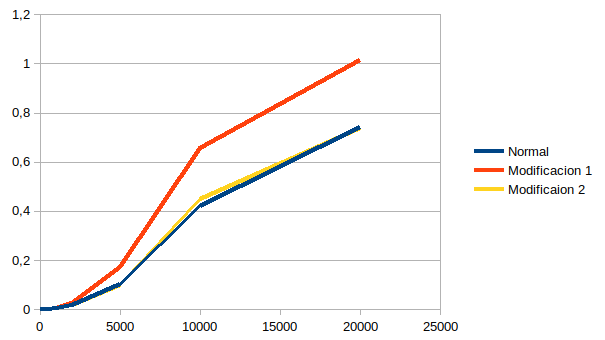
\includegraphics[width=0.7\linewidth]{screenshot001}
	\caption[Comparaci�n 16x16]{Comparaci�n 16x16}
	\label{fig:screenshot001}
\end{figure}\\
El siguiente experimento lo he realizado para tama�os de bloque de $32x32$. Los resultados se pueden ver en la siguiente tabla: \\
\begin{tabular}{|c|c|c|c|}
	\hline 
	N & Original & Modificaci�n 1 & Modificaci�n 2 \\ 
	\hline 
	40 & 0,000056& 0,000056&  0,000046\\ 
	\hline 
	100 & 0,000069 & 0,000096& 0,000086\\ 
	\hline 
	200 &0,000317& 0,000295 &  0,000232\\ 
	\hline 
	500 &0,001090& 0,001570 & 0,001247 \\ 
	\hline 
	1000 & 0,005071 &0,006002 & 0,004240 \\ 
	\hline 
	2000 &0,015409 &0,022229 & 0,017617 \\ 
	\hline 
	5000 &0,093398& 0,177768 & 0,094377 \\ 
	\hline 
	10000 & 0,375558 & 0,665087 &0,407680\\ 
	\hline 
	20000 & 0,881141 & 0,753009 & 0,782449 \\ 
	\hline 
\end{tabular} \\\\
En la Figura \ref{fig:screenshot003} podemos ver la grafica comparando resultados. \\
\begin{figure}[h]
	\centering
	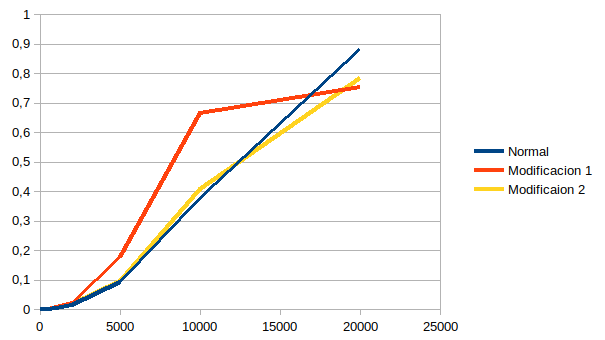
\includegraphics[width=0.7\linewidth]{screenshot003}
		\caption[Comparaci�n 32x32]{Comparaci�n 32x32}
	\label{fig:screenshot003}
\end{figure}\\

Viendo los resultados de tiempo de los experimentos realizados podemos concluir que la mejor opci�n seria usar un tama�o de bloque de $16x16$ con la modificaci�n 2.  Aunque para asegurarnos de estos datos habr�a que haber realizado varios experimentos para el mismo tama�o de bloque y el mismo tama�o de matriz. Otra cosa que podemos deducir de los experimentos realizados es que la peor opci�n es usar la modificaci�n numero 1 en todos los casos. Mientras que en la modificaci�n 2 y en la original obtenemos datos muy parecidos. \\
\end{document}